\chapter{Ostatní zdroje trénovacích dat}
\label{kap:svolocz}

Trénovacích dat pro rozpoznávání řeči není nikdy dost. V~době psaní tohoto textu
je manuálně přepsaných asi 100 hodin z~Mluveného korpusu Karla Makoně. To je pro
natrénování modelu pro jednoho mluvčího použitelné množství a takto dosažená WER
je 20\%. Zda by více trénovacích dat od jiných mluvčích mohlo pomoci, je však
otevřená otázka.

Veřejně k~dispozici je několik zdrojů trénovacích dat pro účely trénování
rozpoznávače češtiny, jichž jsem si vědom:
\begin{itemize}
\item{
    Vystadial\cite{vystadialarticle} se 77 hodinami záznamů internetových
    rozhovorů\cite{vystadialdata},
}
\item{
    The Prague Database of Spoken Czech\cite{pdtscarticle} se 122 hodinami
    spontánních dialogů anotovaných na několika úrovních\cite{pdtscdata},
}
\item{
    Korpus expresivní mluvy COMPANION s~5 hodinami namluvenými jednou
    profesionální mluvčí\cite{companiondata},
}
\item{
    Otázky Václava Moravce: 35 hodin přepsaných záznamů české talk
    show\cite{ovmdata},
}
\item{
    STAZKA: 35 hodin záznamů z~vozidel na silnicích obsahujících anotované
    promluvy\cite{stazkadata},
}
\item{
    88 hodin automaticky přepsaných záznamů z~jednání poslanecké
    sněmovny\cite{pspdata}.
}
\end{itemize}
Celkem se tak dostaneme přibližně na 350 hodin dalších trénovacích dat.

Ze záznamů jednání poslanecké sněmovny však existují také ruční stenografické
přepisy. Velká část jednání a jejich přepisů je veřejně ke stažení na webových
stránkách poslanecké sněmovny. Pokusil jsem se proto z~těchto dat připravit
korpus pro trénování rozpoznávání řeči.

\section{Příprava dat}

Ruční přepisy jednání poslanecké sněmovny jsou, pokud je mi známo, k~dispozici
pouze ve formátu čitelném pro člověka. Přepisy nejsou ve zdrojovém kódu webové
stránky nijak oddělené a jsou promíchané s~metainformacemi. Je tedy nutné
extrakci pojmout jako aproximační úkol. Používám velice jednoduchý algoritmus,
který má své nedostatky, ale pokrývá drtivou většinu záznamů. Extrahuji podstrom
všech elementů s~hodnotou atributu \texttt{[align=justify]} vyjma elementů
\texttt{<b>}, neboť ty obsahují jména mluvčích.

Známé nedostatky spočívají jednak v~tom, že se jména mluvčích sice správně z~přepisu
oddělují, ale navzdory jejich hodnotě coby metainformace zahazují, a jednak
v~tom, že se z~přepisu vynechávají odkazy na jiné schůze. Ty jsou totiž
formátované jinak než ostatní části, jak je vidět např. v~přepisu schůze z 12.
února 2020 od
10:10\footnote{https://www.psp.cz/eknih/2017ps/stenprot/040schuz/s040372.htm}.
Opravení obého je otázkou napsání chytřejšího scraperu a pro účely vybudování
korpusu pro tréning rozpoznávání řeči je obé bezvýznamné: Označení mluvčích
z~principu, vynechání odkazů pro jejich řídkost.

\subsection{Zarovnávání}
\label{subsec:svolocz:zarovnavani}

Jedna z~překážek použití stenografických přepisu pro trénování rozpoznávačů řeči
je velmi volné párování neboli zarovnání přepisů ke zvuku. Každý zvukový záznam
má 14 minut a překrývá se se sousedními čtyři minuty na každé straně.
Přepisy jsou rozdělené na úseky odpovídající těmto záznamům. Zarovnání je tedy
do desetiminutových bloků s~dvouminutovým přesahem na každé straně. Na
obrázku~\ref{fig:svolocz:overlap} je vyobrazeno schéma tohoto apriorního
zarovnání.

\begin{figure}[htpb]
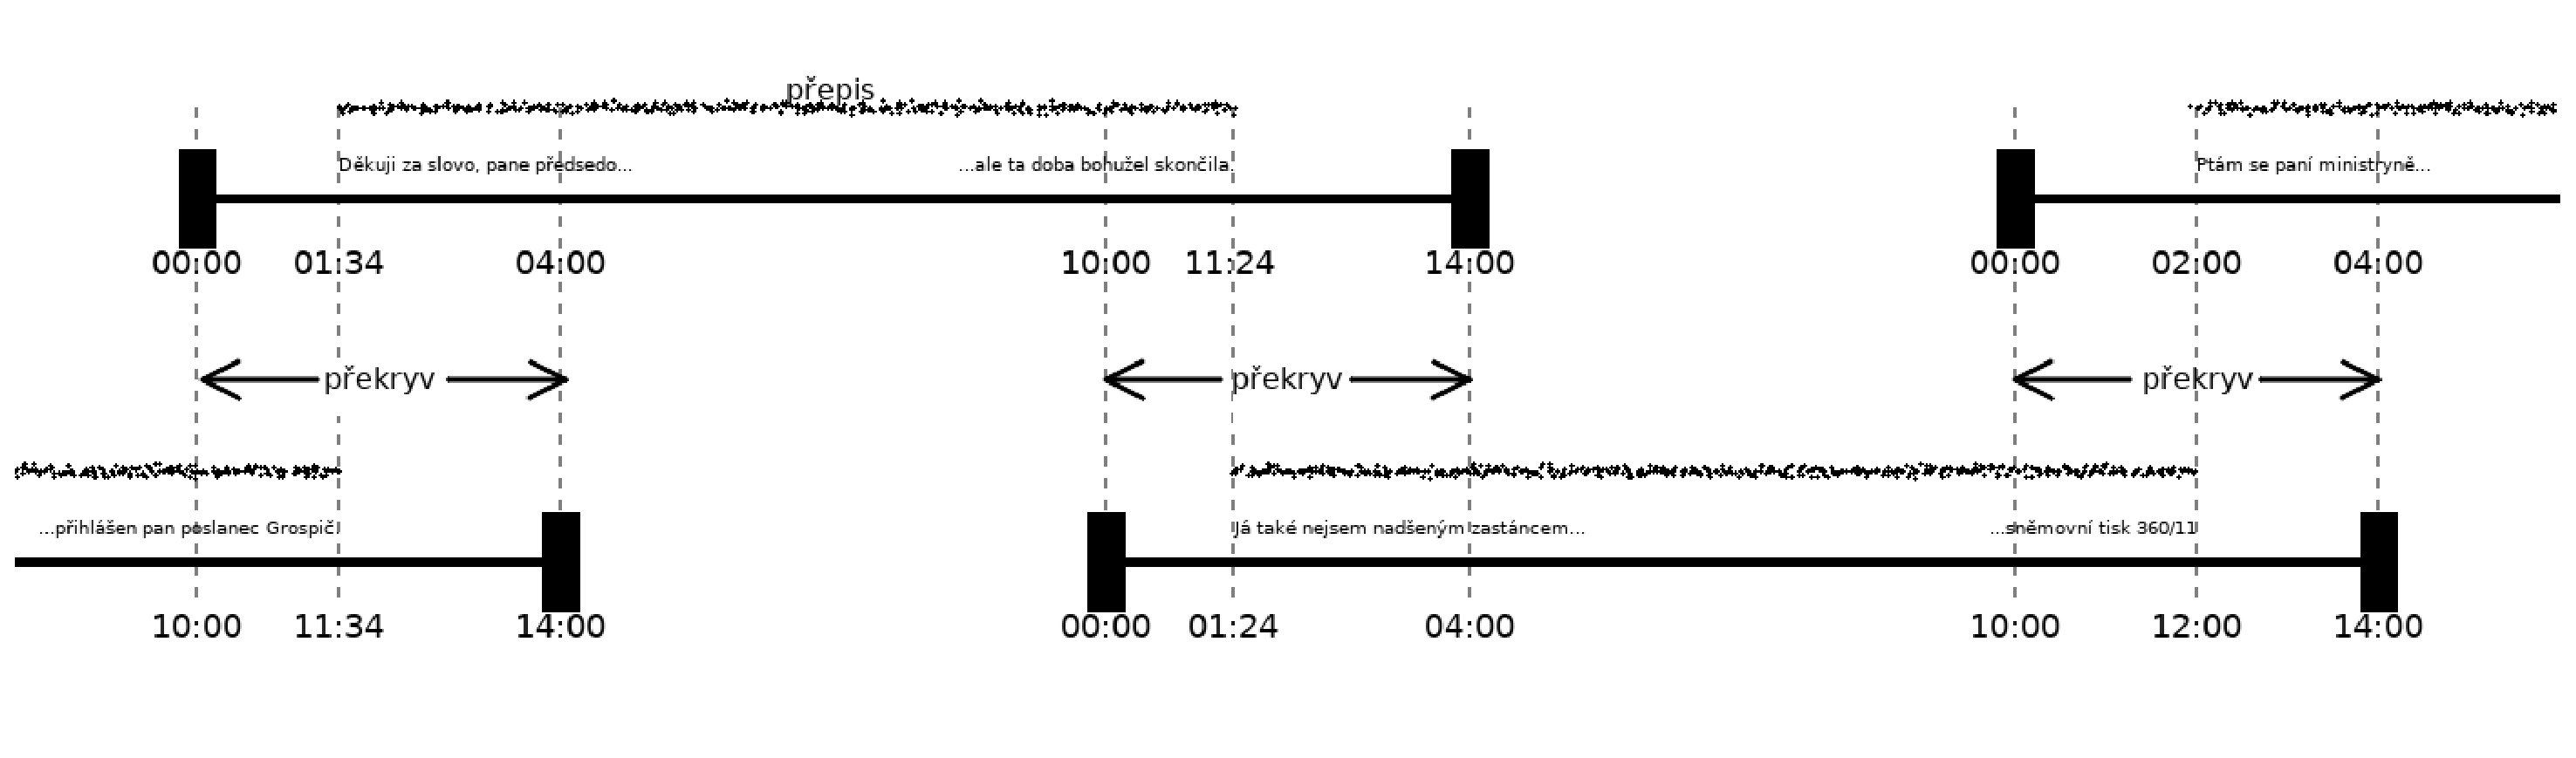
\includegraphics[scale=0.25]{rc/svolocz-overlap.eps}
\caption{Apriorní zarovnání a překruv zvukových záznamů k~přepisům. Vyobrazen je
záznam z 12. února 2020 kolem 10. hodiny. Přepis záznamu vlevo nahoře pokrývá
pozice od 01:34 do 11:24. Vpravo dole pak od 01:24 do 12:00.}
\label{fig:svolocz:overlap}
\end{figure}

Systémů pro zarovnávání dlouhých zvukových záznamů existuje několik, publikovali
je např. Moreno et al\cite{moreno1998recursive} nebo
Hazen\cite{hazen2006automatic}. Oba jsou založeny na využití předem získaného a
zarovnaného automatického přepisu. Taktéž tento přistup využívám, ale
zjednodušený a přizpůsobený úloze.

Za použití výše zmíněného datasetu\cite{pspdata} jsem natrénoval markovovský
akustický model obdobný tomu, jenž je popsán v~kapitole~\ref{kap:asr}. Jazykový
model jsem natrénoval ze stažených stenografických přepisů. Těch je podstatně
víc než nahrávek, protože z~mně neznámého důvodu je valná část odkazů na zvukové
záznamy nefunkčních, končíc chybovým kódem 404 nebo v~menším počtu případů 403.

Pro celý korpus jsem pomocí programu julius vygeneroval automatický přepis se
zarovnáním. Automaticky vygenerovaný zarovnaný přepis každého záznamu jsem pak
porovnal s~odovídajícím manuálním přepisem pomocí Levenshteinovy metody počítání
editačních operací. Zjistil jsem samotné editační operace pro přechod
z~automatického přepisu k~manuálnímu a pro každé slovo v~automatickém přepisu
spočetl, kolik úprav naň připadá. Na základě toho definuji pro každé automaticky
vygenerované slovo spolehlivost párování se slovem manuálně zapsaným jako
\begin{equation}1 - \frac{počet editačních operací}{počet písmen}\end{equation}

Obrázek~\ref{fig:svolocz:align} proces zarovnání manuálních přepisů se zvukovým
záznamem zachycuje.

\begin{figure}[htpb]
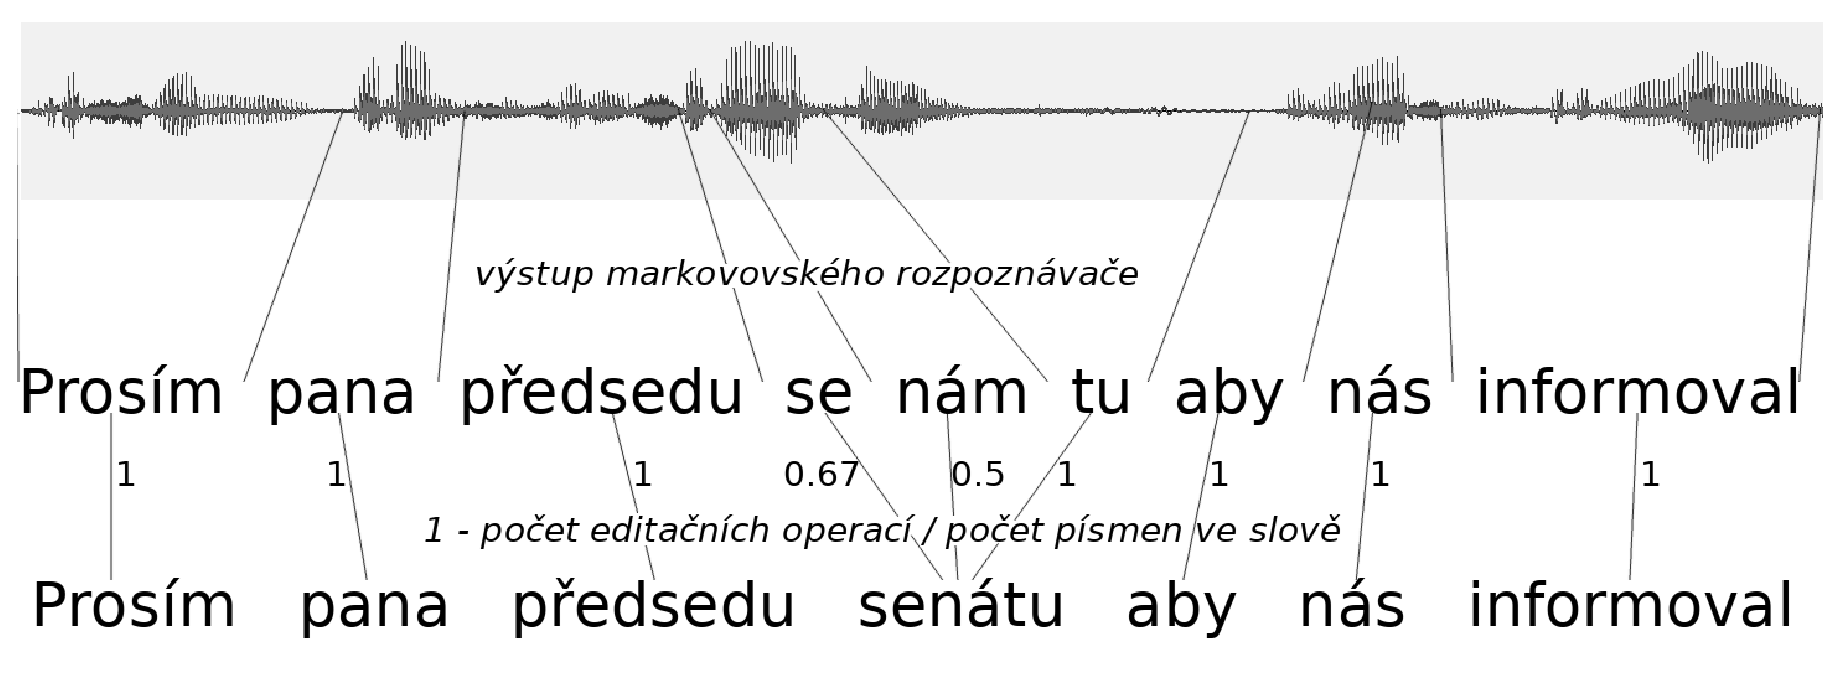
\includegraphics[scale=0.4]{rc/svolocz-align.eps}
\caption{schéma zarovnání zvukových záznamů ke stenografickým přepisům na úrovni
slov}
\label{fig:align}
\end{figure}

\subsection{Tvorba potenciálních trénovacích vzorků}

Kvalita trénovacích dat pro rozpoznávání řeči závisí i na tom, jak jsou
rozdělena. Za prvé je žádoucí, aby byly trénovací vzorky podobně dlouhé
jako testovací vzorky\cite{nagorski2003search}.
V~případě automatického přepisu korpusu Karla Makoně lze
nastavit délku vstupních úseků libovolně. V~obecném případě nelze předvídat.
Za druhé je pro tréning výhodné, aby jednotlivé vzorky měly podobnou délku kvůli
efektivnímu využití operační paměti grafické procesní jednotky. Stačí jeden
dlouhý vzorek a dávka {\em (batch)} způsobí vyčerpání paměti. Naopak mnoho
kraťoučkých vzorků způsobí, že se paměť při dávce zaplní jen málo a plýtvá se
časem. Za třetí, chci-li, aby byla trénovací sada dala použitelná i pro ostatní,
je dobré, aby se délkou vzorků příliš neodlišovala od ostatních datových sad.

Nad to je ale důležité, aby přepis dokonale odpovídal obsahu. A protože
vyřezáváme trénovací vzorky z~delších souborů, při čemž může dojít
k~nepřesnostem, je záhodno volit místa řezu tak, aby padla pokud možno do
delších pauz v~řeči. Je to týž problém jako v~sekci~\ref{sec:segmenty}. V~tomto
případě jsem dospěl k~hranicím 12 - 30 sekund.

\subsection{Výběr trénovacích vzorků}

Po rozdělení desetiminutových nahrávek na úseky vhodné délkou pro trénink je
nutné spárovat tyto úseky s~odpovídajícími úseky manuálních přepisů, a ty, které
jsou spárovány spolehlivě, zařadit do samotné trénovací množiny.
V~podsekci~\ref{subsec:svolocz:zarovnavani} jsem popsal, že máme párování
jednotlivých slov v~automatickém a manuálním přepisu s~určitou mírou
spolehlivosti a že automatický přepis je spárován se zvukovým záznamem. Zbývá
tedy vybrat úseky, které můžeme považovat za spolehlivě přepsané, a zbytek
zahodit.

Nahrávky se překrývají tak, že z~každého čtrnáctiminutového souboru je jen deset
minut pokryto odpovídajícím přepisem, takže zahodit musíme minimálně 40\% úseků.
Dospěl jsem k~následujícím kritériím:

\begin{enumerate}
\item{Spolehlivost prvního a posledního slova v~úseku alespoň 70\%.}
\item{Průměrná spolehlivost všech slov v~úseku alespoň 70\%.}
\item{Alespoň 5 slov v~úseku.}
\end{enumerate}



%           cstest      selftest
% ovm       0.728954    0.216131
% bible     0.947226    0.091958
% cucfgn    0.728446    0.316287
% vystadial 0.739838    0.509930
% svolocz   0.397490    0.083978
% makon     0.773216    0.191772
% oral2013  0.607015    0.783525
% all       0.283574    0.283574
%
% cucfgnOF  0.683059    0.141142
% all\o                 0.130555
